\let\negmedspace\undefined
\let\negthickspace\undefined
\documentclass[journal]{IEEEtran}
\usepackage[a5paper, margin=10mm, onecolumn]{geometry}
%\usepackage{lmodern} % Ensure lmodern is loaded for pdflatex
\usepackage{tfrupee} % Include tfrupee package
\setlength{\headheight}{1cm} % Set the height of the header box
\setlength{\headsep}{0mm}     % Set the distance between the header box and the top of the text
\usepackage{gvv-book}
\usepackage{gvv}
\usepackage{cite}
\usepackage{amsmath,amssymb,amsfonts,amsthm}
\usepackage{algorithmic}
\usepackage{graphicx}
\usepackage{textcomp}
\usepackage{xcolor}
\usepackage{txfonts}
\usepackage{listings}
\usepackage{enumitem}
\usepackage{mathtools}
\usepackage{gensymb}
\usepackage{comment}
\usepackage[breaklinks=true]{hyperref}
\usepackage{tkz-euclide} 
\usepackage{listings}
% \usepackage{gvv}                                        
\def\inputGnumericTable{}                                 
\usepackage[latin1]{inputenc}                                
\usepackage{color}                                            
\usepackage{array}                                            
\usepackage{longtable}                                       
\usepackage{calc}                                             
\usepackage{multirow}                                         
\usepackage{hhline}                                           
\usepackage{ifthen}                                           
\usepackage{lscape}
\renewcommand{\thefigure}{\theenumi}
\renewcommand{\thetable}{\theenumi}
\setlength{\intextsep}{10pt} % Space between text and floats
\numberwithin{equation}{enumi}
\numberwithin{figure}{enumi}
\renewcommand{\thetable}{\theenumi}
\begin{document}
\bibliographystyle{IEEEtran}
\title{11.16.3.11}
\author{EE24BTECH11006- Arnav Mahishi}
% \maketitle
% \newpage
% \bigskip
{\let\newpage\relax\maketitle}
\textbf{Question:-} In a lottery, a person chooses six different natural numbers at random from 1 to 20, and if these six numbers match with the six numbers aldready fixed by the lotttery committee, he wins a prize. What is the probability of winning the prize in the game?
\textbf{Solution: }\\
The sample space is 
\begin{align}
  \Omega &= \sbrak{\text{All possible collections of 6 numbers from 1 to 20}}\\
  \implies\abs{\Omega}&=\binom{20}{6}
\end{align}
Assuming equally likely outcomes, 
\begin{align}
  \Pr\brak{\omega \in \Omega} = \frac{1}{\abs{\Omega}}=\frac{1}{\binom{20}{6}}
\end{align}
Let X represent the event:\newline
X=1, The person wins the prize (All the numbers match)\\
X=0: The person does not win (numbers don't match).\\
The Probability Mass Function (PMF) for the given random variable is
\begin{align}
P(X = k) =
\begin{cases}
	1-\frac{1}{\binom{20}{6}}, & k = 0 \\
	\frac{1}{\binom{20}{6}}, & k = 1 \\
\end{cases}
\end{align}
The Cumulative Distribution Function (CDF) for the given random variable is
\begin{align}
F_X(k) = P(X \le k) = 
\begin{cases}
	0, & k < 0 \\
	1-\frac{1}{\binom{20}{6}}, & 0 \le k < 1 \\
	1, & k \le 1\\
\end{cases}
\end{align}
The probability of winnig the lottery is
\begin{align}
  \Pr\brak{X=1} &= \frac{1}{\binom{20}{6}}
\end{align}
\textbf{Simulation}

To simulate the lottery, the process follows these steps:

\begin{enumerate}
    \item \textbf{Random Number Generation:} Generate random numbers uniformly from 1 to 20 for both the player and the committee using a uniform random number generator.
    
    \item \textbf{Simulate Multiple Trials:} Run the simulation for a large number of trials (e.g., 1,000,000), where in each trial the player's six numbers are compared to the committee's six numbers.
    
    \item \textbf{Match Calculation:} If all six numbers match, the player wins. The number of wins is tracked.
    \item \textbf{Probability Calculation:} Calculate the probability of winning as the ratio of winning trials to total trials. The true probability is \( \frac{1}{\binom{20}{6}} \).

    \item \textbf{Relative Frequency:} Track and plot the relative frequency of winning over time to observe convergence to the true probability.

    \item \textbf{Final Results:} After all trials, generate:
    \begin{itemize}
        \item Probability Mass Function (PMF)
        \item Cumulative Distribution Function (CDF)
        \item Convergence of relative frequency to the true probability
    \end{itemize}
\end{enumerate}

The following shows how the relative frequency reaches true probability with increasing number of trials of the event.
\newpage
\begin{figure}[h!]
   \centering
   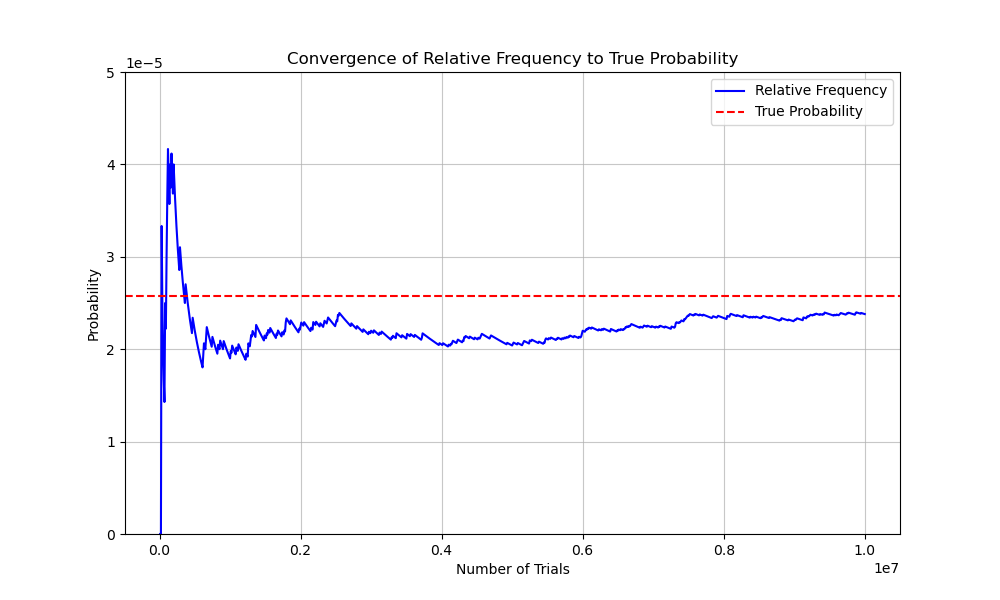
\includegraphics[width=1\columnwidth]{figs/fig.png}
    \caption{Relative Frequency tends to True Probability}
\end{figure}
\begin{figure}[h!]
   \centering
   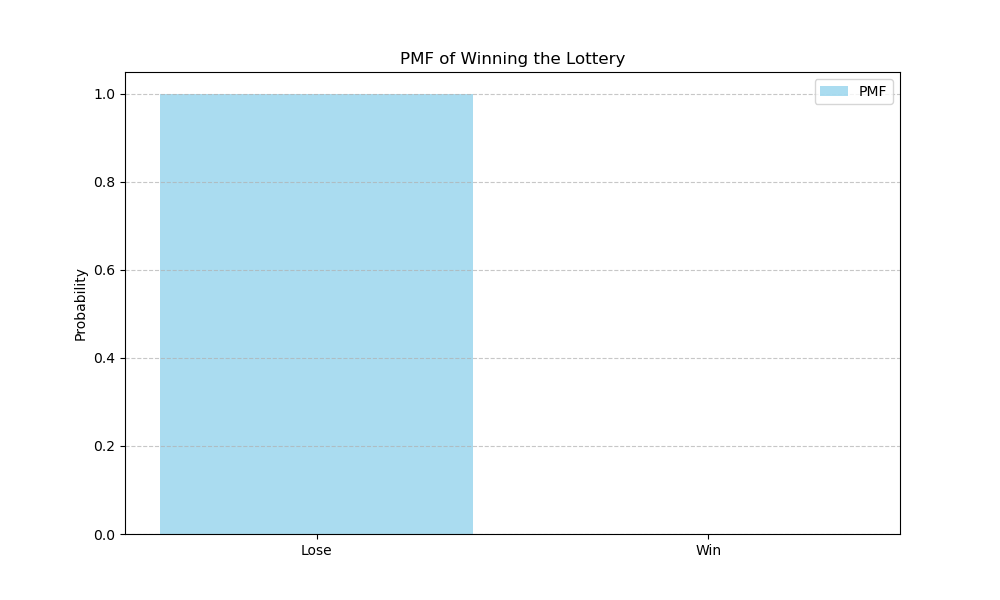
\includegraphics[width=1\columnwidth]{figs/pmf.png}
    \caption{Probability Mass Function of given Random variable}
\end{figure}
\newpage
\begin{figure}[H]
   \centering
   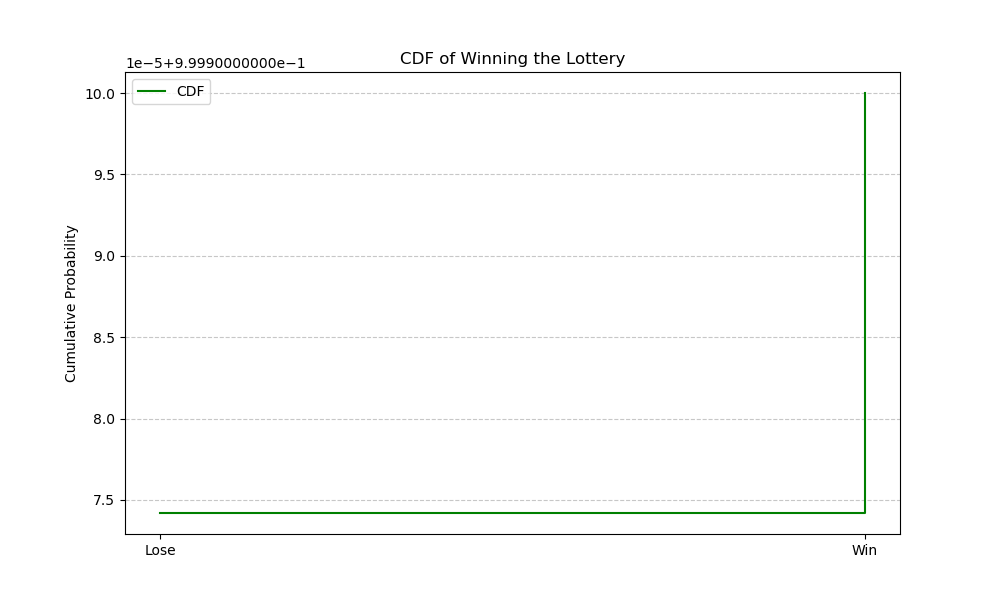
\includegraphics[width=1\columnwidth]{figs/cdf.png}
    \caption{Cumulative Distribution Function of given Random variable}
\end{figure}
\end{document}
